% Make nice A4 pages for print:
%\usepackage{pgfpages}
%\pgfpagesuselayout{resize to}[a4paper,border shrink=5mm,landscape]

\beamertemplatenavigationsymbolsempty

\setbeamertemplate{bibliography item}[text]

\usepackage[type={CC},modifier={by-sa},version={4.0}]{doclicense}

\usepackage[utf8]{inputenc}
\usepackage{hyperref}
\usepackage{breakurl}
\usepackage{graphicx}
\usepackage{pgfplots}
\usepackage{pgf}
\usepackage{tikz}
\usetikzlibrary{positioning}
\usetikzlibrary{arrows}
\usetikzlibrary{decorations.markings}
\usetikzlibrary{calc}
\usetikzlibrary{matrix}
\usetikzlibrary{shapes}
\usetikzlibrary{decorations.pathmorphing}
\usetikzlibrary{fit}
\usetikzlibrary{backgrounds}
\usetikzlibrary{plotmarks}
\usepackage{stmaryrd}
\usepackage{listings}
\usepackage{pdflscape}
\usepackage{perpage}
\usepackage{appendixnumberbeamer}

%\usepackage[thmmarks,amsmath,amsthm]{ntheorem} % already included in beamer
\usepackage{thm-restate}

\usepackage[sort&compress,numbers]{natbib}  % to be have \citet, \citeauthor, \citeyear

\MakePerPage{footnote}

\tikzstyle{o}=[r,ppBlue]
\tikzstyle{r}=[thick,rectangle,align=center]
\tikzstyle{t}=[r,ppTrans] %,font=\bfseries]
\tikzstyle{dd}=[densely dashed]
\tikzstyle{n}=[r,ppBlue]
\tikzstyle{p}=[r,ppRed]
\tikzstyle{ppRed}  =[draw=red,  fill=  red!20]
\tikzstyle{ppBlue} =[draw=blue, fill= blue!20]
\tikzstyle{ppGreen}=[draw=green,fill=green!20]
\tikzstyle{ppTrans}=[draw=none, fill=none]

\usetheme{Warsaw}

\useoutertheme[subsection=true]{smoothbars}
%\useoutertheme[subsection=false]{miniframes}

\definecolor{bblue}{HTML}{D7DF01}	% yellow-ish actually, for better black/white printing
\definecolor{rred}{HTML}{C0504D}
\definecolor{ggreen}{HTML}{9BBB59}
\definecolor{ppurple}{HTML}{9F4C7C}
\definecolor{lightgray}{rgb}{0.3,0.3,0.3}
\definecolor{lightergray}{rgb}{0.9,0.9,0.9}
\definecolor{UniBlue}{RGB}{83,121,170}

\DeclareTextFontCommand\textintro{\normalfont\bfseries\itshape} % nice!
\newcommand{\intro}[2][]
{%
	\textintro{#2}%
}
\newcommand{\empha}[2][]
{%
	\emph{#2}%
}

%\theoremstyle{plain}
\newcounter{reqcounter}
\newtheorem{requirement}[reqcounter]{Requirement}

%setbeamercolor{structure}{fg=violet}

\makeatletter
\def\th@task{%
    \normalfont % body font
    \setbeamercolor{block title example}{bg=orange,fg=white}
    \setbeamercolor{block body example}{bg=orange!20,fg=black}
    \def\inserttheoremblockenv{exampleblock}
  }
\makeatother

\theoremstyle{task}
\newtheorem{task}{Task}

\newenvironment{assignment}%
{%\setbeamercolor{background canvas}{bg=violet}%
%\setbeamercolor{structure}{fg=cyan!90!black}%
 \setbeamercolor{frametitle}{bg=orange,fg=white}
\begin{frame}}%
{\end{frame}}%

\AtBeginSection[]{
  \begin{frame}
  \vfill
  \centering
  \begin{beamercolorbox}[sep=8pt,center,shadow=true,rounded=true]{title}
    \usebeamerfont{title}\insertsectionhead\par%
  \end{beamercolorbox}
  \tableofcontents
  \vfill
  \end{frame}
}




\pgfplotsset{compat=1.14}
\author{Markus Raab}


\title{LRE Recapitulation}
\date{23.06.2021}

\begin{document}


%%%%%%%%%%%%%%%%%%%%%%%%%%%%%%%%%%%%%%%%%% 
\section{Recapitulation}

\begin{frame}
	\frametitle{Metalevels}
	\begin{alertblock}{Question}
	Describe the three Metalevels in Elektra and CM.
	\end{alertblock}

	\pause
	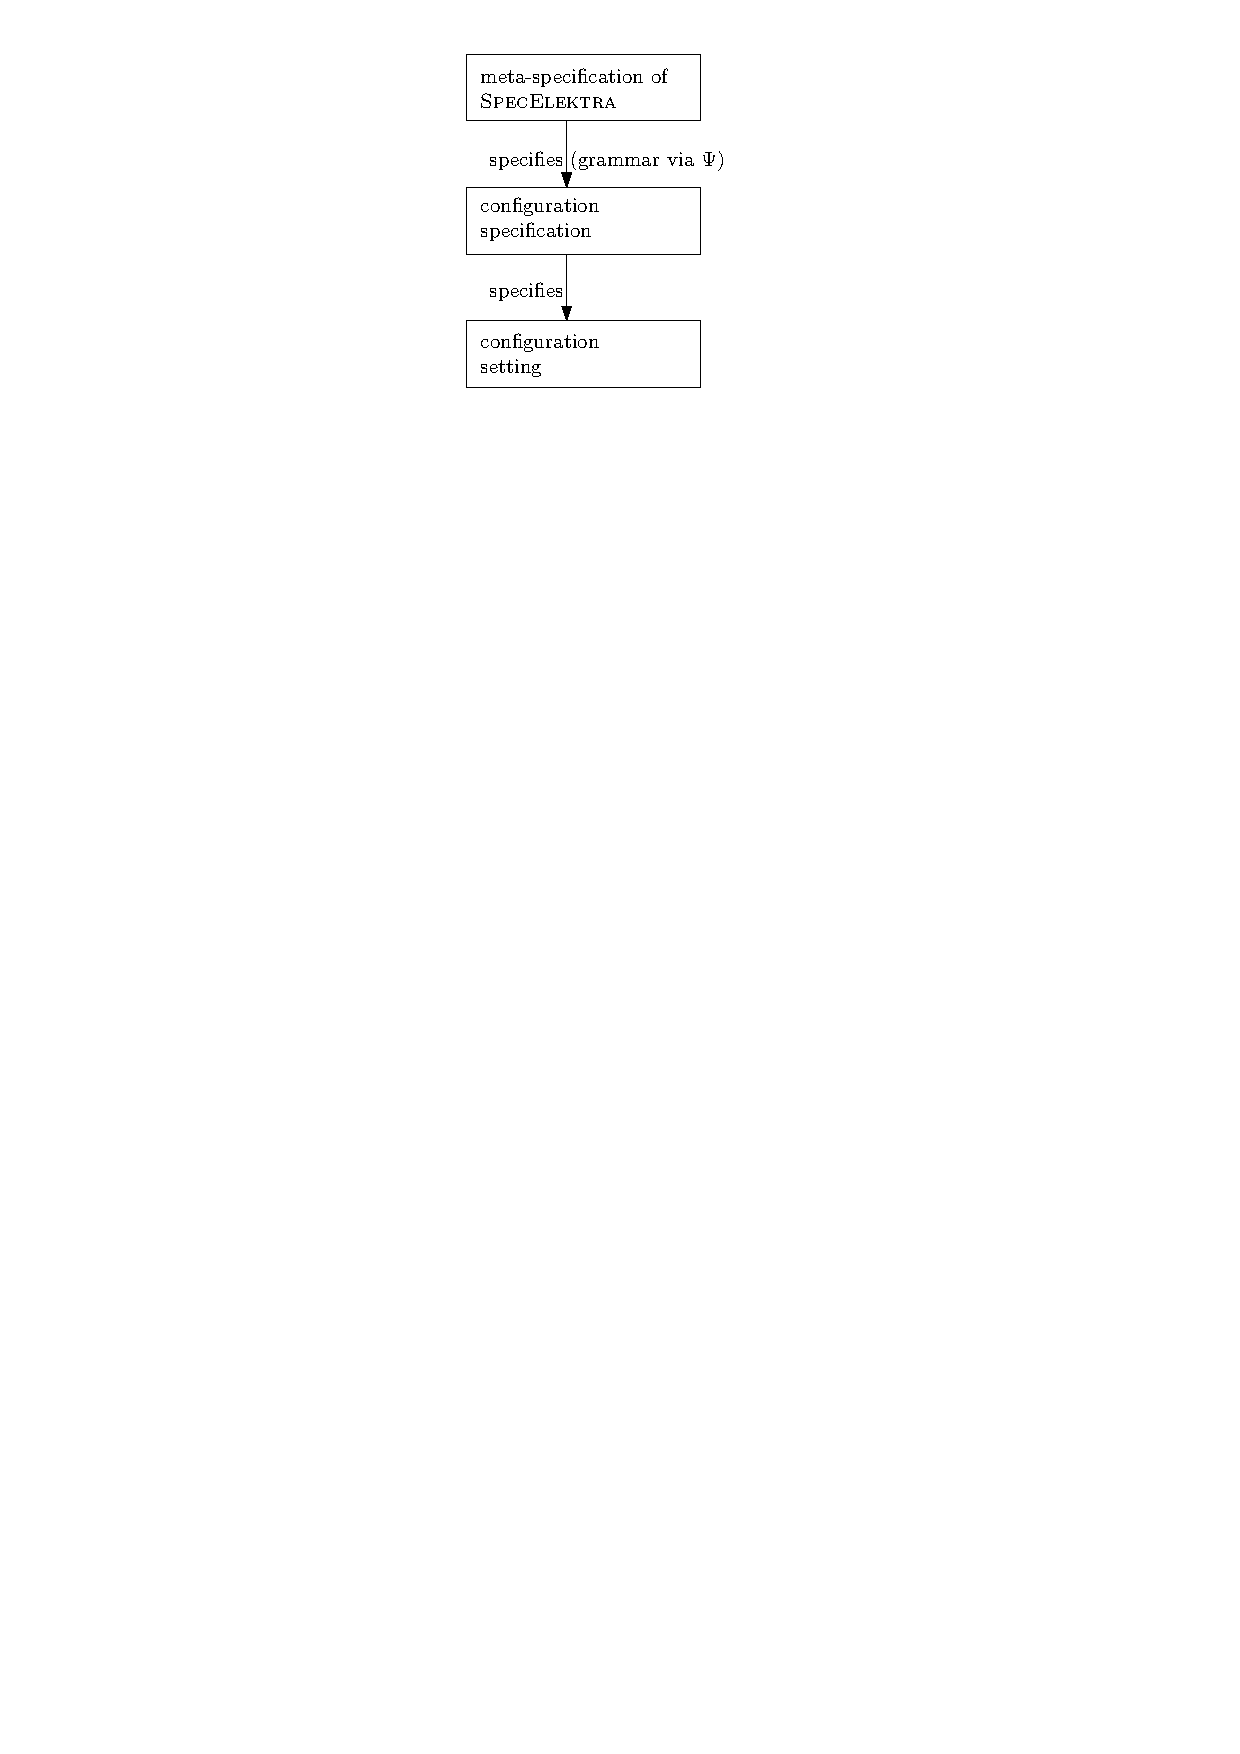
\includegraphics{metalevels}
\end{frame}

\begin{frame}
	\frametitle{Integration: Current Situation}

	\pause
	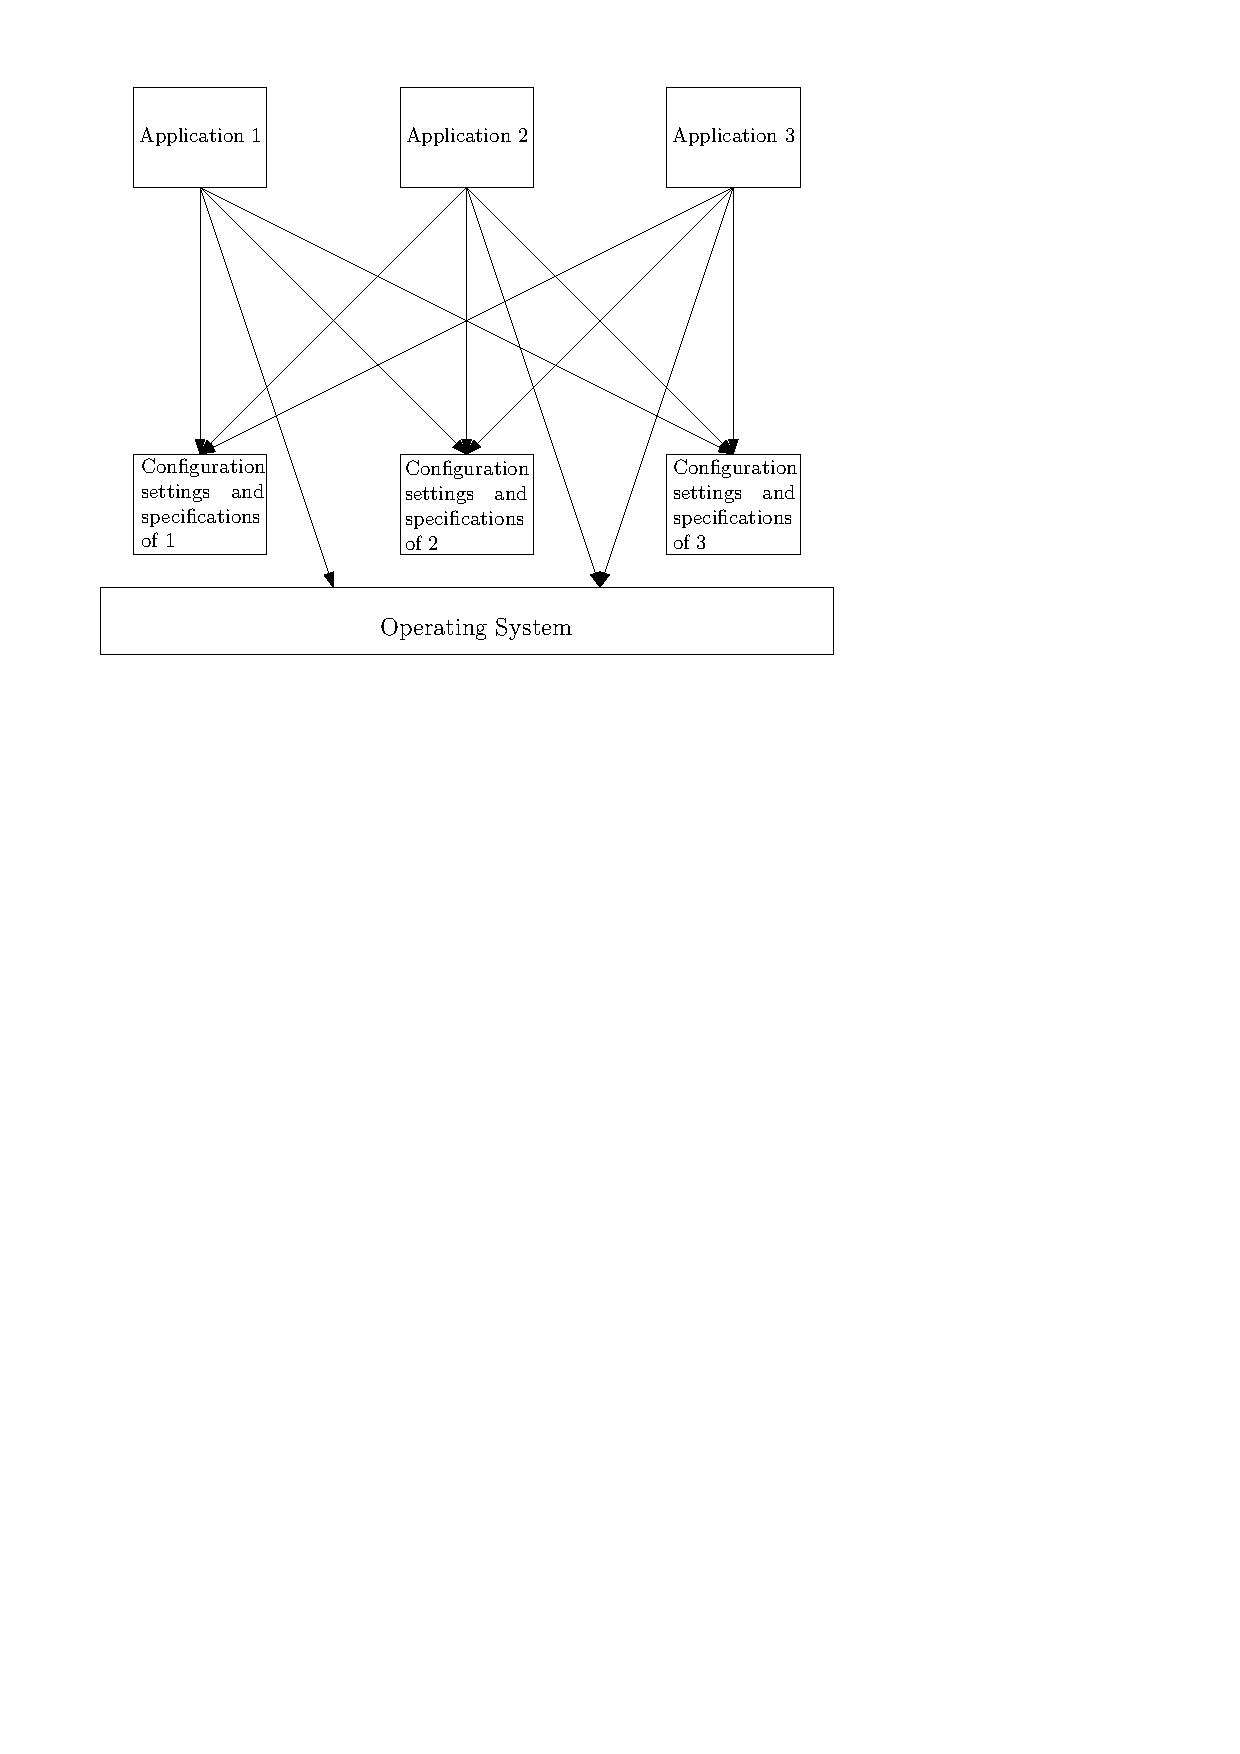
\includegraphics[scale=0.7]{cursituation}
\end{frame}

\begin{frame}
	\frametitle{Integration: Wanted Situation}

	\pause
	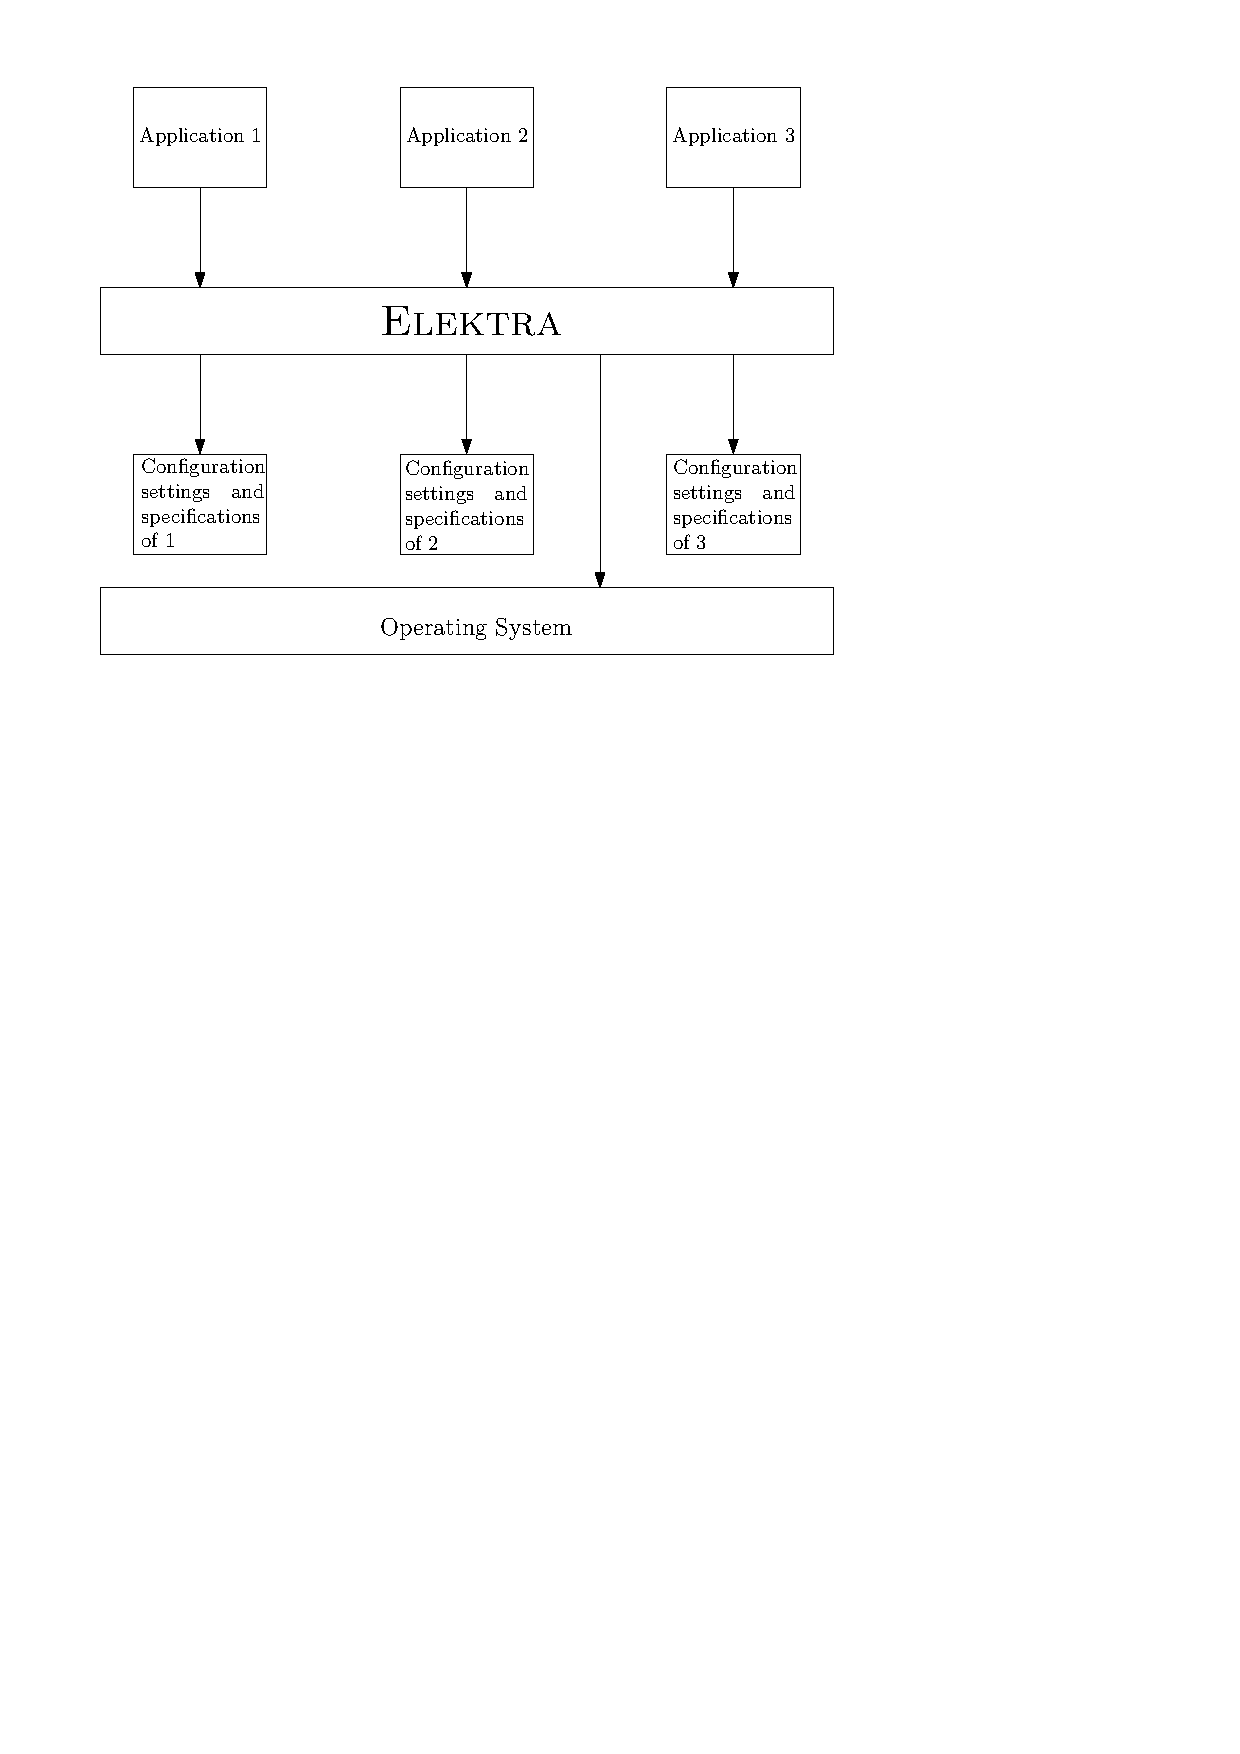
\includegraphics[scale=0.7]{wantsituation}
\end{frame}

\begin{frame}
	\frametitle{Possible Benefits of CM}

	\begin{task}
	What are the goals of CM Tools?
	\end{task}

	\pause

	\begin{itemize} %[<+-| alert@+>]
	\item The same goals scripts have: \\
		Documentation, Customization, Reproducability
	\item Declarative description of the system \\
		Single Source of Truth 
		(Infrastructure as Code~\cite{waldemar2013testing})
	\item Less configuration drift
	\item Error handling
	\item Pull vs.\ Push
	\item Reusability
	%\item (Resource) Abstractions
	\end{itemize}
\end{frame}

\begin{frame}
	\frametitle{Develop CM-aware applications}

	\begin{task}
	What needs to be considered by developers to make applications CM-aware?
	\end{task}

	\pause[\thebeamerpauses]  %  show after \begin{itemize}[<+->]

	\begin{itemize} %[<+-| alert@+>]
	\item reduce the configuration complexity
	\item intensively review and improve the specifications
	\item test (and debug) different configuration settings
	\item allow introspection
	\item consider context
	\end{itemize}
\end{frame}

%\breakframe

\section{Conclusion}

\begin{frame}
	\frametitle{Popular Topics 2022S}
	\vspace{-0.55cm}
	\setlength{\columnsep}{-1.3cm}
	\raggedright
	\definecolor{amethyst}{rgb}{0.6, 0.4, 0.8}
	\begin{multicols}{2}
	\begin{description}
	\item[6] {\color{amethyst} CM-Tools: Ansible}
	\item[4] {\color{amethyst} Context Awareness} % Collected in L10
	\item[3] {\color{amethyst} Design Configuration} % Collected in L10
	\item[3] {\color{amethyst} Validation}
	\item[3] {\color{amethyst} configuration versioning}
	\item[2] {\color{gray} Spring Initializr (https://start.spring.io/)}
	\item[2] {\color{amethyst} Specification and Integration}
	\item[2] {\color{red} Kubernetes CM}
	\item[2] {\color{amethyst} Integration (Common view on different configuration sources)}
	\item[2] {\color{amethyst} Infrastructure CM}
	\item[1] {\color{gray} Docker Compose YAML}
	\end{description}
	\end{multicols}
\end{frame}

\begin{frame}
	\frametitle{Learning Outcomes (TISS)}
	Students will be able to

	\begin{enumerate}
	% Technical and Methodological Knowledge
	\item support configuration management during software engineering,
	\item describe systematic approaches for configuration management and exemplary configuration management tools.
	%Cognitive and Practical Skills
	\item use configuration specification languages,
	\item implement such specified variability during program construction,
	\item apply techniques of quality assurance in configurable applications.
	% Social and Personal Skills
	\item communicate variability with system administrators.
	\end{enumerate}
\end{frame}

\begin{frame}
	\tiny
	\frametitle{Learning Outcomes}
	Students will be able to

	\begin{itemize}
	% L01
	\item remember definitions of configuration settings.
	% TODO: meta-levels
	($\rightarrow$ TISS 2)

	% L02
	\item use configuration specification languages.
	(= TISS 3)

	% L03
	\item remember strategies for configuration integration.
	($\rightarrow$ TISS 1)

	% L04
	\item differentiate between configuration sources.
	($\rightarrow$ TISS 1)
	\item unify configuration sources via specifications.
	($\rightarrow$ TISS 1)

	% L05
	%\item {\color{gray} write simple configuration management scripts.}
	\item describe systematic approaches for configuration management and exemplary configuration management tools.
	($=$ TISS 2)

	% L06
	\item write simple checker plugins.
	($\rightarrow$ TISS 4)

	% L07
	\item remember terms of properties of CM.
	($\rightarrow$ TISS 2)
	\item remember various strategies for reduction of misconfiguration.
	%\item find unused settings.
	($\rightarrow$ TISS 2)
	($\rightarrow$ TISS 5)

	% L08
	\item recall points of time relevant in configuration management.
	%\item remind some arguments about pull vs.\ push.
	%\item remember various strategies for earlier reduction of misconfiguration.
	($\rightarrow$ TISS 5)

	% L09
	%\item recall a method of avoiding errors.
	\item apply some principles of good error messages.
	($\rightarrow$ TISS 5)
	\item remind some basics of system administrator research.
	($\rightarrow$ TISS 6)

	% L10
	\item design and document configuration settings and specifications.
	($\rightarrow$ TISS 1)
	\item evaluate a configuration system and decide about use of
	($\rightarrow$ TISS 5)
	\begin{itemize}
	\tiny
	\item code generation.
	\item introspection.
	\item context-awareness.
	\end{itemize}

	% L11
	\item remember connections between the many different topics within CM.
	\end{itemize}
\end{frame}

\begin{frame}
	\frametitle{Map}

	\vspace{-0.5cm}
	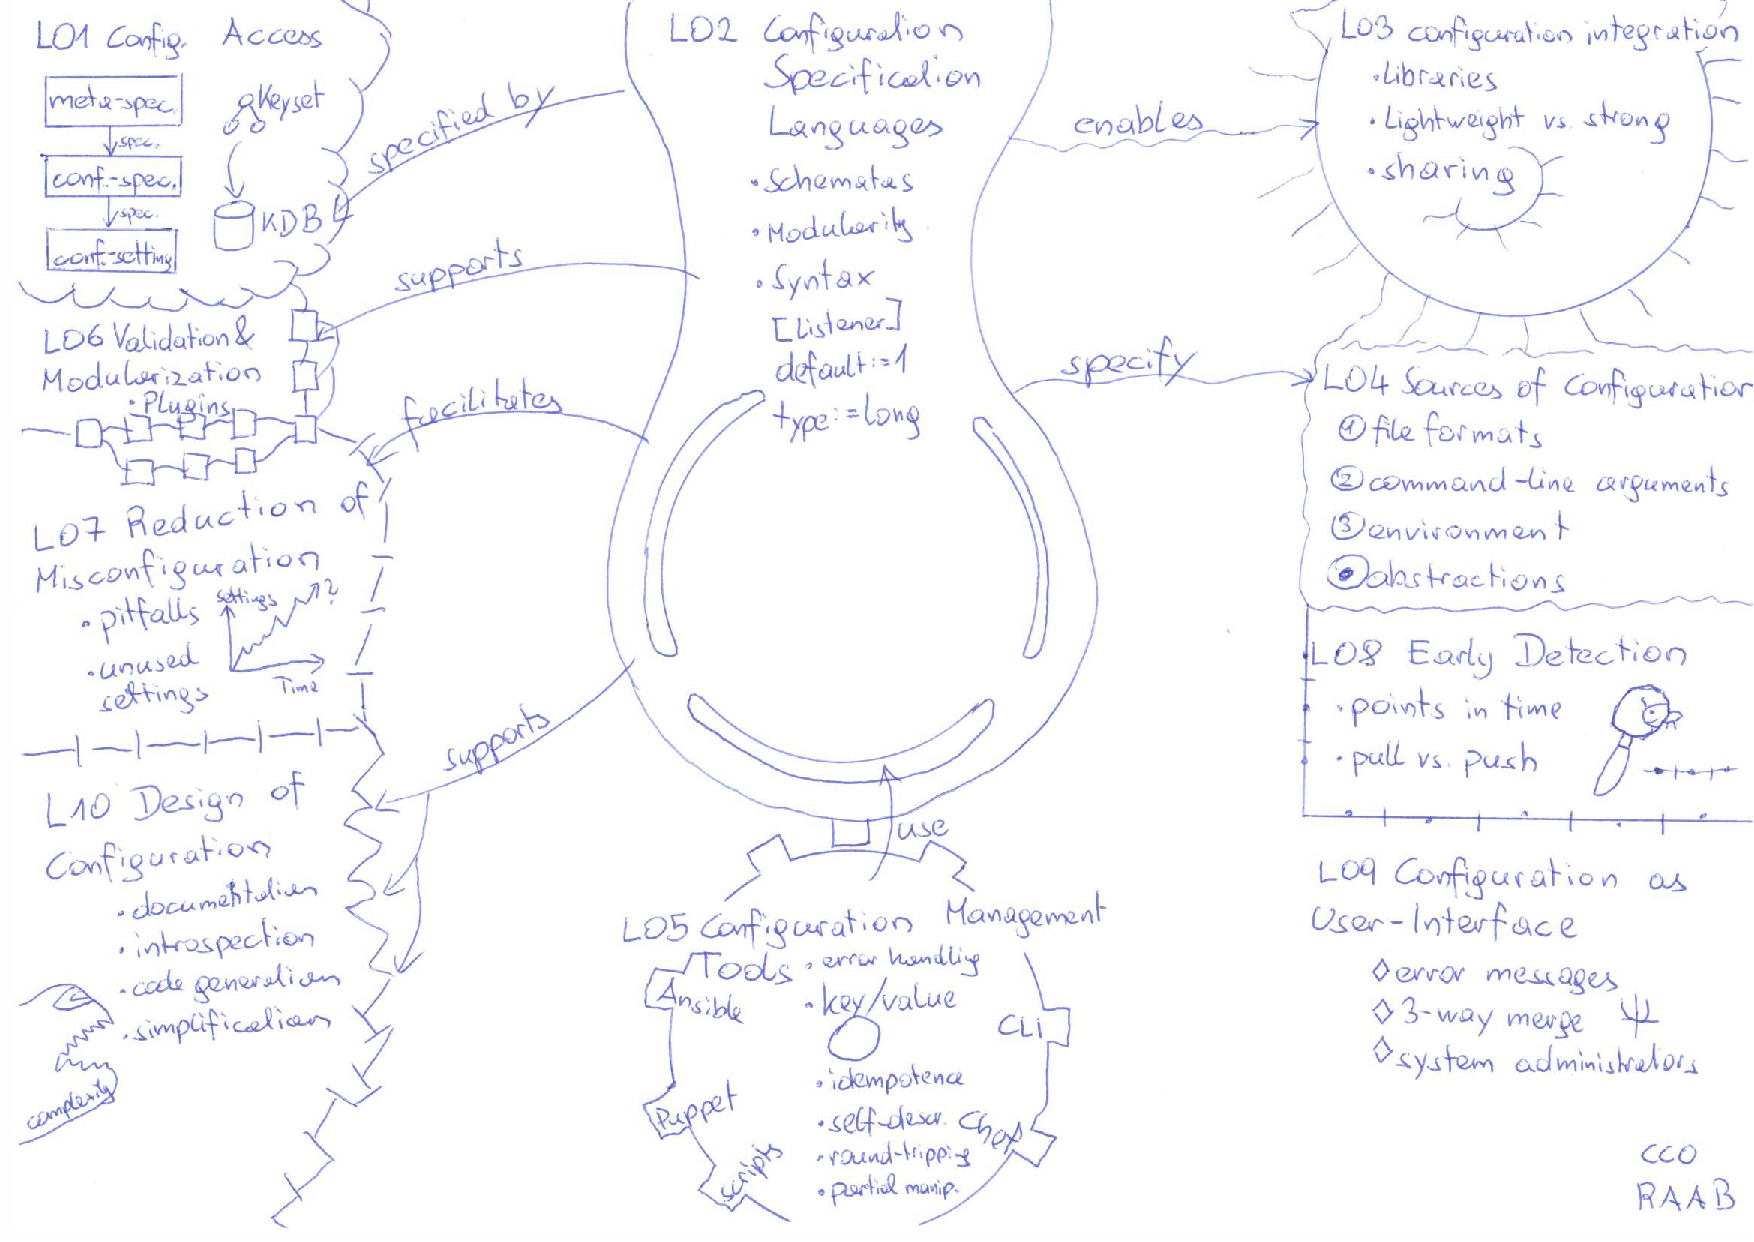
\includegraphics[width=8cm]{pics/map.pdf}
\end{frame}

\section{Preview}


\begin{frame}
	\frametitle{Feedback}
	\hfill \includegraphics[width=2cm]{pics/feedback.png}
	\vspace{-1cm}
	\begin{itemize}
		\item TUWEL Feedback %\linebreak
		%{\scriptsize \url{https://tuwel.tuwien.ac.at/mod/feedback/view.php?id=1259052}}
		\vspace{0.2cm}
		\item TISS Feedback \linebreak
		{\small from 16.06.2022 00:00 until 14.07.2022 23:59
		\scriptsize \url{https://tiss.tuwien.ac.at/survey/surveyForm.xhtml?courseNumber=194030&semesterCode=2022S}}
	\end{itemize}
\end{frame}

\begin{frame}
	\frametitle{Conclusion}

	Doing CM is easier if the applications support it.
	\vspace{1cm}

	I hope the lecture helped you to know how to write such applications.
\end{frame}




%%%%%%%%%%%%%%%%%%%%%%%%%%%%%%%%%%%%%%%%%% 
\nocite{raab2017introducing}

\appendix

\begin{frame}[allowframebreaks]
	\bibliographystyle{plainnat}
	\bibliography{../shared/elektra.bib}
\end{frame}

\end{document}

